\documentclass[12pt,reqno]{amsart}
\usepackage{./header}

\hdr{Mathematical Statistics}{Chapter 1: Probability spaces}

\begin{document}

\bigskip

\prob Let $A$ and $B$ be two subsets of a set $S$. Let $C$ be the subset of $S$ consisting of elements that are in $A$ or $B$, but not both. Express $C$ in terms of $A$ and $B$ using only the basic set operations.
\vspace{2in}

















\prob Draw Venn diagrams to illustrate \text{DeMorgan's law}, which states that, given two subsets $A$ and $B$ of a set $S$, that

	\[(A\cup B)^c = A^c \cap B^c.\]
\vspace{2in}












\prob Identify appropriate sample spaces for each of the following scenarios.

\medskip
\begin{enumerate}
\item Rolling a die.\vfill
\item Flipping a coin.\vfill
\item Flipping a coin \textit{three} times.\vfill
\item Flipping a coin until it lands heads.\vfill
\item Forecasting whether it will rain tomorrow.\vfill
\item Conducting an experiment to measure the speed of light.\vfill
\end{enumerate}











\newpage
\prob Describe some events in the following scenarios. Use the sample spaces that you identified in the previous problem.

\medskip
\begin{enumerate}
\item Rolling a die.\vfill
\item Flipping a coin.\vfill
\item Flipping a coin \textit{three} times.\vfill
\item Flipping a coin until it lands heads.\vfill
\item Forecasting whether it will rain tomorrow.\vfill
\item Conducting an experiment to measure the speed of light.\vfill
\end{enumerate}












\prob Suppose that you choose at random one of the twelve months of the year.

\medskip
\begin{enumerate}
\item Identify an appropriate sample space.\vfill
\item Identify the event that you choose a month beginning with a ``J''.\vfill
\item Identify the event that you choose a month whose name is four letters long.\vfill
\item Using one of the basic set operations and your answers to the two previous parts, identify the event that you choose a month beginning with a ``J'' and whose name is four letters long.\vfill
\end{enumerate}

























\prob Suppose that $A$ and $B$ are two events. Write expressions involving only the basic set operations for each of the following:

\bigskip
\begin{enumerate}
\item Both events occur.\vfill
\item At least one occurs.\vfill
\item Neither occurs.\vfill
\item Exactly one occurs.\vfill
\end{enumerate}














\newpage
\prob Let $P$ be the discrete probability measure on the sample space $S=\mathbb{R}$ with probability mass function

	\[
	p(s) = \begin{cases}
	1/4 & : s=0, \\
	1/4 & : s=2, \\
	1/2 & : s=4, \\
	0 & : \text{otherwise}.
	\end{cases}
	\]

Compute the probabilities $P(A)$ of the following events.

\medskip
\begin{enumerate}
\item $A = [-2, -1]$\vfill
\item $A = (-1, 1)$\vfill
\item $A = (-1, 1) \cup (3,5]$\vfill
\item $A = \mathbb{R}$\vfill
\end{enumerate}













\prob Let $P$ be the discrete probability measure on the sample space $S=\mathbb{R}$ with probability mass function

	\[
	p(s) = \begin{cases}
    	(0.25) (0.75)^{s-1} & : s=1, 2, 3, \ldots, \\
	0 & : \text{otherwise}.
	\end{cases}
	\]

Compute the probabilities $P(A)$ of the following events.

\medskip
\begin{enumerate}
\item $A = (-\infty,1)$\vfill
\item $A = (-10, 4]$\vfill
\item $A = \mathbb{R}$\vfill
\item $A = \{\text{all positive even integers}\}$\vfill
\end{enumerate}
















\newpage
\prob Describe in complete detail a probability space that models each of the following scenarios. Be sure to check that the two requirements in the Discrete Probability Construction Lemma are both satisfied.

\medskip
\begin{enumerate}
\item Rolling a fair six-sided die.\vfill
\item Flipping an \textbf{unfair} coin, with probability $0.25$ of obtaining heads, and probability $0.75$ of obtaining tails.\vfill
\item Flipping an \textbf{unfair} coin twice, with probability $0.25$ of obtaining heads, and probability $0.75$ of obtaining tails. What is the probability that you flip \textit{exactly} one head?\vfill
\item Flipping an \textbf{unfair} fair coin until you obtain a head, with probability $0.25$ of obtaining heads, and probability $0.75$ of obtaining tails. What is the probability that you flip an odd number of tails before you see a head?\vfill
\end{enumerate}


















\prob A sample space consists of five simple events, $E_1$, $E_2$, $E_3$, $E_4$, and $E_5$.

\medskip
\begin{enumerate}
\item If $P(E_1) = P(E_2) = 0.15$, $P(E_3) = 0.4$, and $P(E_4) = 2P(E_5)$, find the probabilities of $E_4$ and $E_5$.\vfill
\item If $P(E_1) = 3P(E_2) = 0.3$, find the probabilities of the remaining simple events if you know that the remaining simple events are equally probable.\vfill
\end{enumerate}















\newpage
\prob A survey classified a large number of adults according to whether they were diagnosed as needing eyeglasses to correct their reading vision and whether they use eyeglasses when reading. The proportions falling into the four resulting categories are given in the following table:

\medskip
\begin{center}
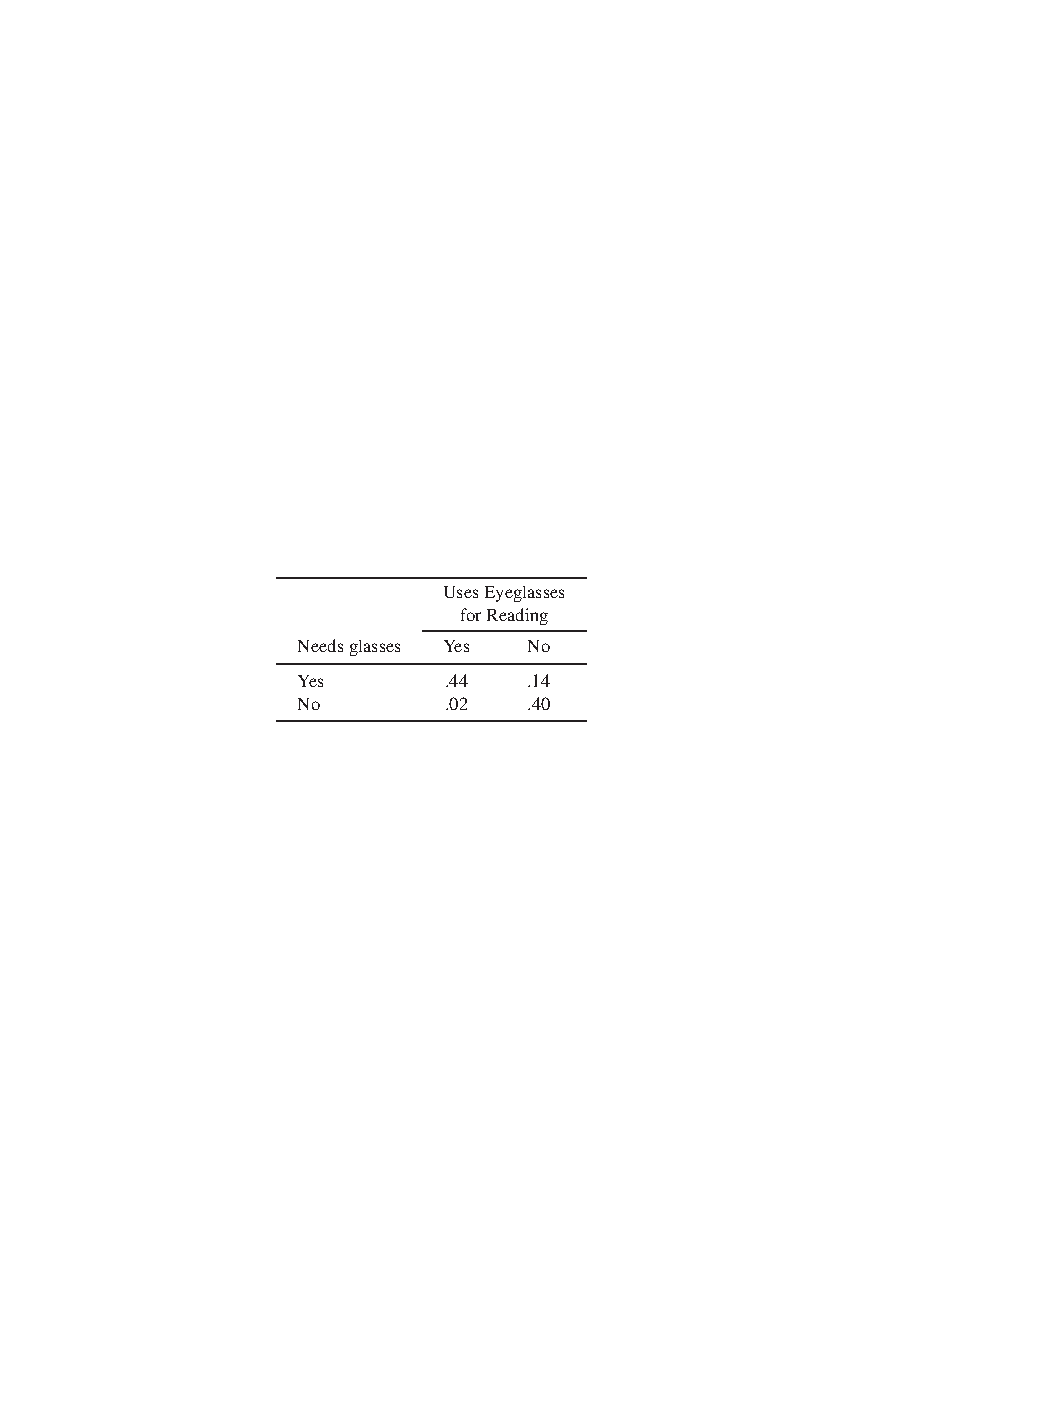
\includegraphics[scale=1]{img.pdf}
\end{center}
\medskip

If a single adult is selected from the large group, find the probabilities of the events defined below. The adult

\medskip
\begin{enumerate}
\item needs glasses.\vfill
\item needs glasses but does not use them.\vfill
\item uses glasses whether the glasses are needed or not.\vfill
\end{enumerate}















\prob Let $P$ be a continuous probability measure on the sample space $S=\mathbb{R}$ with probability density function

	\[
	f(s) = \begin{cases}
	\frac{2}{9}s & : 0 \leq s \leq 3, \\\
	0 & : \text{otherwise}.    
	\end{cases}
	\]

Compute the probabilities $P(A)$ of the following events.

\medskip
\begin{enumerate}
\item $A=(-1, 1]$\vfill
\item $A = (-1,1) \cup [2, 4)$.\vfill
\item $A = [0,3]$.\vfill
\item $A = \mathbb{R}$.\vfill
\end{enumerate}











\newpage
\prob Let $P$ be a continuous probability measure on the sample space $S=\mathbb{R}$ with probability density function

	\[
	f(s) = \begin{cases}
	\displaystyle\frac{1}{s^2} & : s \geq 1, \\\
	0 & : \text{otherwise}.    
	\end{cases}
	\]

Compute the probabilities $P(A)$ of the following events.

\medskip
\begin{enumerate}
\item $A=(-10, 0)$\vfill
\item $A = \mathbb{R}$.\vfill
\end{enumerate}









\prob A particle is located somewhere along the real line $\mathbb{R}$, but the \text{only} information that you have about its location is that it is at some point in the interval $[0,4]$.

\medskip
\begin{enumerate}
\item Describe in complete detail a probability space that models this scenario.\vfill
\item Suppose some new information comes to light that suggests the particle is closer to $4$ than it is $0$. Alter your probability model to reflect this new information.\vfill
\end{enumerate}
    













\newpage
\prob Let $P$ be the discrete probability measure on $\mathbb{R}$ with probability function

	\[
	p(s) = \begin{cases}
	\frac{2!}{s!(2-s)!} \left( \frac{1}{4} \right)^s \left(\frac{3}{4} \right)^{2-s} & : s=0, 1, 2, \\
	0 & :\text{otherwise}.
    	\end{cases}
	\]

Compute the distribution function $F(s)$.\vfill
















\prob Let $P$ be the continuous probability measure on $\mathbb{R}$ with density function

	\[f(s) = \begin{cases}
	3s^2 & : 0 \leq s \leq 1, \\
	0 & : \text{otherwise}.
	\end{cases}
	\]

Compute the distribution function $F(s)$.\vfill
















\prob Let $P$ be a probability measure on $\mathbb{R}$ with distribution function

	\[
	F(s) = \begin{cases}
	0 & : s < 0, \\
	s & : 0\leq s \leq 1, \\
	1 & : s>1.
	\end{cases}
	\]

Is $P$ continuous? If so, compute its density function $f(s)$.\vfill


















\newpage
\prob Let $P$ be the discrete probability measure on $\mathbb{R}$ with probability function

	\[
	p(s) = \begin{cases}
	3/8 & : s=1, \\
	7/16 & : s=2, \\
	3/16 & : s=3, \\
	0 & : \text{otherwise}.
	\end{cases}
	\]

Compute the following quantiles:

\medskip
\begin{enumerate}
\item $Q(0.25)$\vfill
\item $Q(0.5)$ (the median of $P$)\vfill
\item $Q(0.75)$\vfill
\end{enumerate}












\prob Let $P$ be the continuous probability measure on $\mathbb{R}$ with density function

	\[f(s) = \begin{cases}
	cs(1-s) & : 0 \leq s \leq 1, \\
	0 & : \text{otherwise}.
	\end{cases}
	\]

\medskip
\begin{enumerate}
\item Find the value of $c$ that makes $f(s)$ a valid density function.\vfill
\item Compute the quantile $Q(0.95)$.\vfill
\end{enumerate}












\newpage
\prob Let $P$ be a continuous probability measure on the sample space $S=\mathbb{R}^2$ with probability density function

	\[
	f(s,t) = \begin{cases}
	\frac{1}{8}(s+t) & : 0\leq s,t \leq 2, \\
	0 & : \text{otherwise}.    
	\end{cases}
	\]

Compute the probabilities $P(C)$ of the following events.

\medskip
\begin{enumerate}
\item $C=[-1,1] \times (-1,1)$\vfill
\item $C = \mathbb{R}^2$.\vfill
\end{enumerate}












\prob Let $P$ be a continuous probability measure on the sample space $S=\mathbb{R}^2$ with probability density function

	\[
	f(s,t) = \begin{cases}
	e^{-(s+t)} & : s,t >0, \\
	0 & : \text{otherwise}.    
	\end{cases}
	\]

Show that $P(\mathbb{R}^2)=1$.\vfill

















\newpage
\prob A particle is now located somewhere in the plane $\mathbb{R}^2$, but the \text{only} information that you have about its location is that it is at some point in the square

	\[
	R = [0,3] \times [0,3].
	\]

\medskip
\begin{enumerate}
\item Describe in complete detail a probability space that models this scenario.\vfill
\item Suppose some new information comes to light that suggests the particle is closer to the corner $(3,3)$ than to the origin $(0,0)$. Alter your probability model to reflect this new information.\vfill
\end{enumerate}
    
   
\end{document}